\chapter{Artifact Design - Components of a Modular Classification Pipeline}
\section{Overview}
\label{sec:overview}
In this chapter we deinfe all the components for an end-to-end text classification pipeline built on a robust ETL foundation, a layered data layout, and a lightweight ML layer with continuous learning. It specifies how raw data moves from diverse sources into a staging area, is transformed into reliable, queryable datasets, and is then used to train, evaluate, serve, and continually update a classifier without compromising data integrity or lineage.

\section{ETL Pipeline Design}

This section presents a clear ETL design for turning mixed source data into reliable, ready to use datasets. We begin with careful extraction guided by a simple data map and field level profiling so we pull only the fields we need without slowing source systems. Next, transformation cleans and standardizes the inputs, enforces schemas and types, handles missing values and duplicates, and logs any quality issues for later review. Finally, loading writes the results into partitioned, well defined tables, first with a one time backfill and then with regular incremental runs. The goal is a reproducible and traceable data that analytics and model training can trust. Here are the core components of the ETL design:

\subsection{Extraction}
The Extract-Transform-Load (ETL) begins with extraction. That means accessing one or more source systems to retrieve the data needed for downstream processing , and transferring it to a staging area \cite{mandala:2019} . The primary goal is to pull the required data with minimal impact on the sources, which means without degrading their performance response time or causing locks \cite{gjcs:2023}. Data sources can include transactional apps (CRM/ERP), APIs , files and IoT sensors. They can deliver data in different formats like :  relational tables, JSON , XML and logs. Data volumes may also vary widely depending on the business context.
\smallskip

That's why before building any extract job, define what to extract and why at a logical level. You can achieve this by producing a logical data map. A logical data map defines for each data field , their business meaning , original source and transformation rules \cite{kimball:2004}. After we have defined which data is necessary for the organization we list the systems and APIs likely to contain the required information. The next step after listing the sources that contain the required data , these data elements are then profiled in order to extract the necessary fields for the business need. Data in each source must be analyzed and each field must be profiled to determine its data type , unique identifiers , table relationships and cardinalities. As the final step of extraction , the pipeline determines which changes to pull from each source. After profiling , not every column is relevant , so the extractor should retrieve only the needed fields. The best query returns exactly what you need and not an entire table to be trimmed later \cite{kimball:2004}. In order to capture new or changed data we can query based on \texttt{updated\_at} field. The result of this stage is data with relevant fields selected and change rules defined and it's now ready for Transformation.
The ETL Pipline steps are shown in Figure~\ref{fig:etl_steps}.

\begin{figure}[htbp]
  \centering
  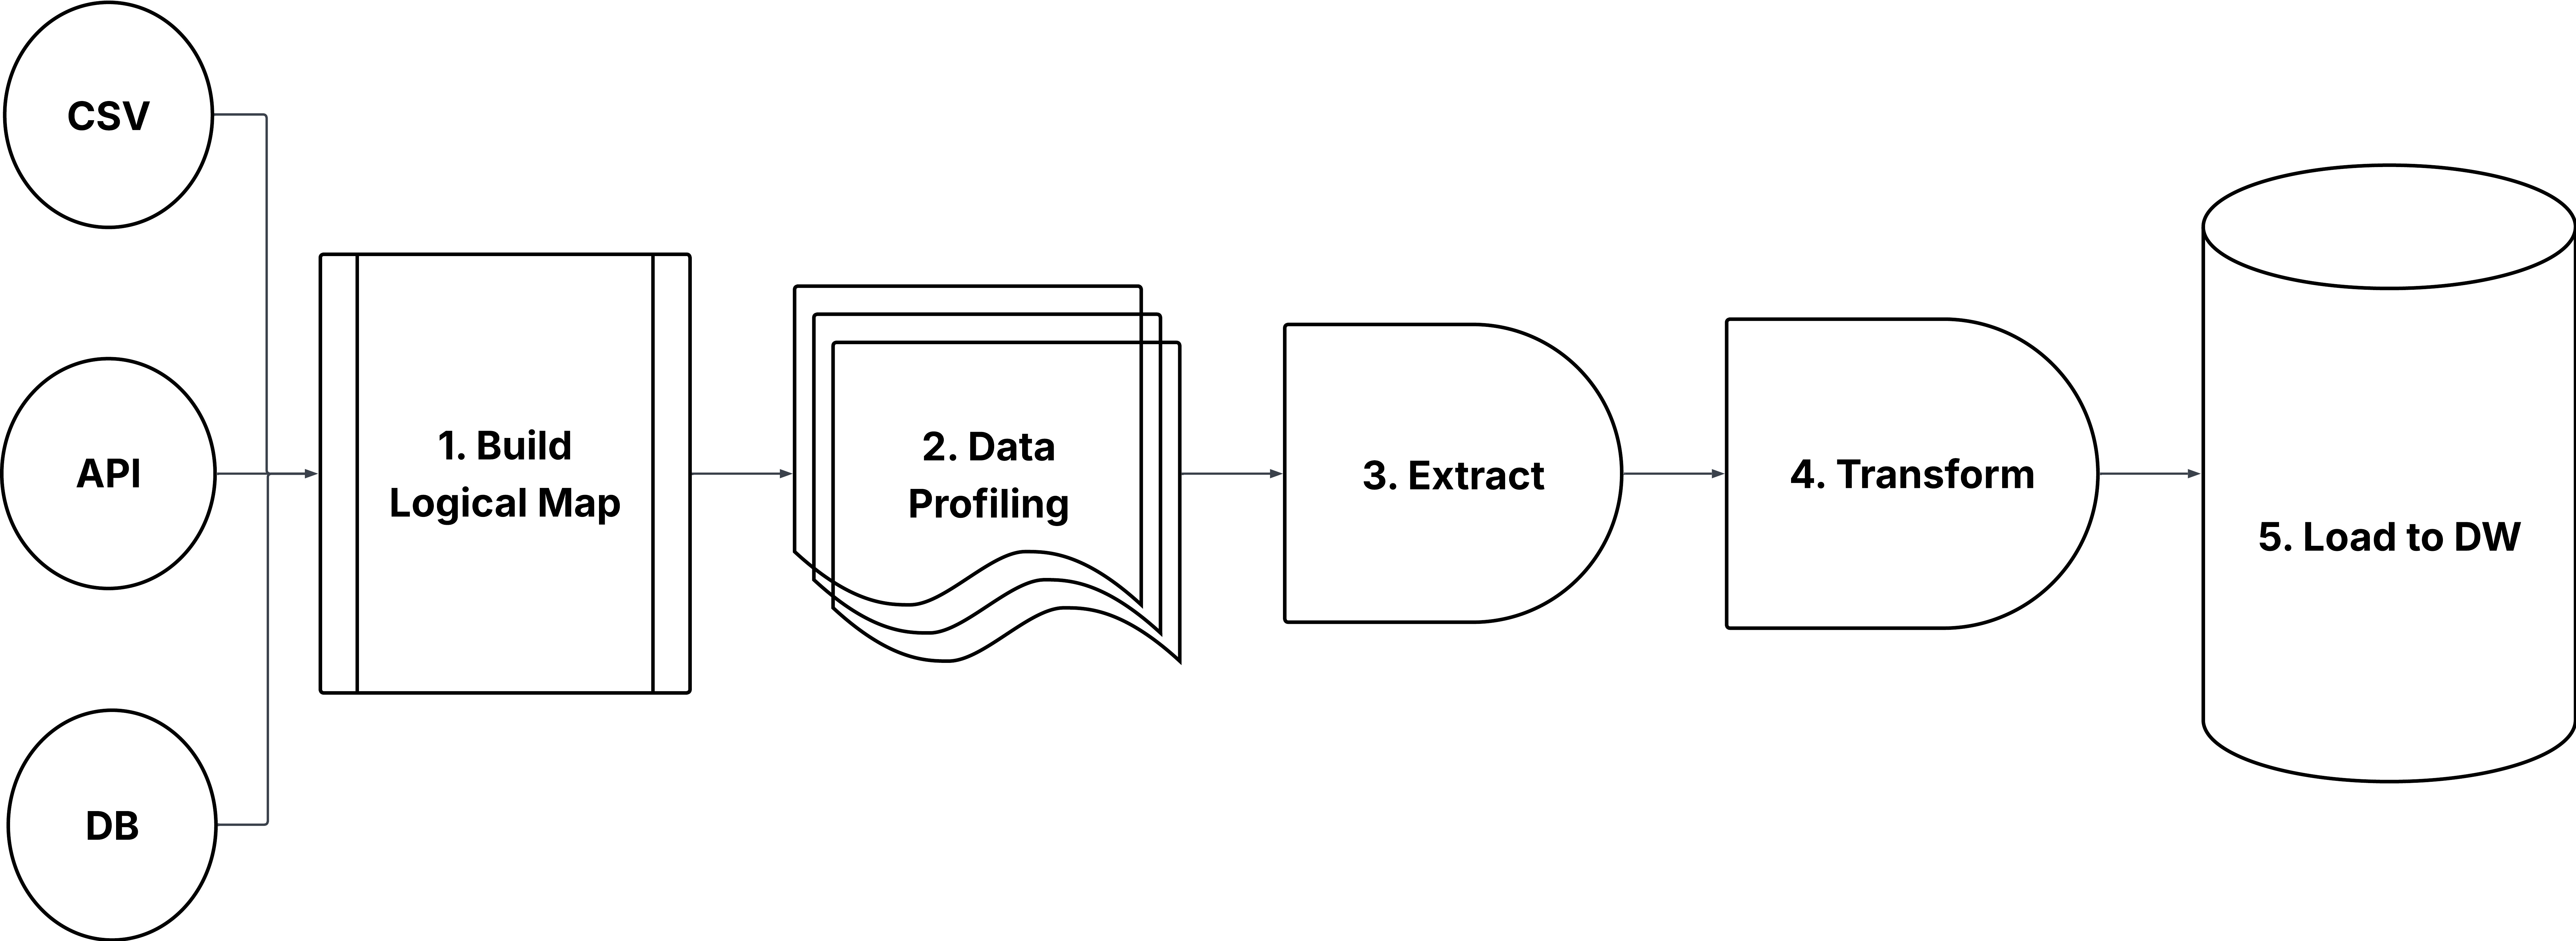
\includegraphics[width=0.8\linewidth]{gfx/examples/etl_steps.jpeg}
  \caption{ETL Pipline Steps.}
  \label{fig:etl_steps}
\end{figure}

\subsection{Transformation}
After extraction , data is standardized so it can be reliably stored and used for serving and modelling \cite{mandala:2019}. In practice , sources are heterogeneous (databases , files , APIs ) and formats vary, that's why a substantial part of analytics work is therefore pre-processing \cite{gjcs:2023} . Cleaning and conforming the data are ETL steps that add the most value , since they decide where the data is fit for purpose and produce metadata , like profiling results and error logs , that should travel with the data. These are the common steps that a transformation step should have \cite{bilal:2022}:

\paragraph{Standard Transformation Rules}
\begin{enumerate}
  \item[\textbf{1.}] \textbf{Standardise fields.} Normalise units like currencies, time zones, whitespaces, phone/email formats, and document any outliers.
  \item[\textbf{2.}] \textbf{Detect \& cast data types.} First infer base types, then re-scan the columns to classify them as native types.
  \item[\textbf{3.}] \textbf{Handle missing values.} Define your missing-values policy. Either leave them null, fill with the most frequent value, mark as ``unknown'', or drop the whole row.
  \item[\textbf{4.}] \textbf{Remove duplicates.} Drop exact duplicates and apply matching rules.
  \item[\textbf{5.}] \textbf{Detect outliers.} Flag extreme values where they would distort the ML model.
  \item[\textbf{6.}] \textbf{Apply calculations.} If the data field requires calculations, apply them before loading into the database.
  \item[\textbf{7.}] \textbf{Log events.} On any rule violation, write an error entry and attach an audit record to the metadata.
\end{enumerate}

\subsection{Loading}
\label{sec:load_patterns}
The loading step writes the transformed data into a central storage used for analytics and serving . In this blueprint , that means building datasets into the warehouse layers that later can be used for users and the ML models for training . Loading is where the pipeline turns intermediate files into queryable , partitioned tables with clear schemas , keys and partitions that jobs can rely on\cite{burgos:2022}. There are two load patterns that are most commonly used:



\begin{description}
  \item[The historical load.] This strategy backfills one or more tables with a large volume of past data, often months or years in a one-time load. This populates the warehouse with existing data before running daily jobs to extract new or changed data. In order to handle large volumes of data, the loading process is usually split into chunks to make it easier to load and less error prone. \cite{kimball:2004}

  \item[The incremental load.] After the first historical backfill, the pipeline switches to incremental loads, which adds new records and apply changes detected since the last run. Incremental behaviour can be append only or upsert (insert new or update existing), depending on the table's purpose. Append only is used for logs and immutable facts and is usually partitioned by date, while upsert is used for changing tables that require frequent updates. \cite{kamat:2022}
\end{description}

Whichever pattern is used , loads should be accurate and record where the data came from. A good load step is predictable and repeatable. Each run targets a known time window or partition and re-running produces the same result. For performance, large batches are written into the storage using bulk loaders and often in parallel by partition. \cite{kimball:2004}

With this behavior in place, the warehouse becomes a stable repository , ready to serve data for monitoring , analytics , training and business consumption.





\section{Data Warehouse Layer Design - Medallion architecture}
To keep the pipeline modular and make data accessible across each stage of transformation, we organize it into three logical layers. This “Medallion” pattern exposes data at each step of the transformation process, so producers and consumers of data will work against different interfaces instead of a single storage. Because of this architecture pattern , data quality improves at each layer. If a mistake occurs and some data is removed , we can always trace it back. In addition , this layered approach enables easier access control , so that different groups of people can be restricted to consume only specific layers \cite{wiselka:2024}. The result is a clear separation of concerns with simpler change management and better lineage of data.

\subsection{Bronze Layer}
Bronze Layer stores raw ingested data in its raw original format \cite{mohna:2022} . In this stage the raw data is stored along other ingestion metadata. This includes fields like \texttt{run\_id}, \texttt{ingest\_batch\_id}, \texttt{source}, \texttt{retrieved\_at}, and \texttt{unique\_identifier}. Loading strategy for bronze data is append only , that means once loaded into storage the data remains immutable. The data is typically partitioned by retrieved time or source that was extracted from \cite{gujjala:2024}. Because Bronze layer holds large volumes of raw data that we rarely directly read from , its main value that this layer adds is traceability and auditability. When needed , we can pull records from a specific day/week/monthor by source , making it easy to reconstruct past states without touching downstream layers \cite{gujjala:2024}. Minimal or no transformation happens during the bronze loading of data.

\subsection{Silver Layer}
The silver layer cleans and standardizes the captured raw data and turn them into tables ready to be used in analytics. At this stage , the pipeline enforces schema rules , cast types , fills in missing values , removes duplicates and applies semantic normalisation. It also performs essential data integration so that unstructured or semi-structured inputs become reliable and queryable formats \cite{nieto:2019}. Silver layer resolves data quality issues and prepares conformed datasets for downstream loading and modelling. It presents a consumption focused view that may power real-time dashboard or predictive services

\subsection{Gold Layer}
The gold layer delivers curated datasets for Business Intelligence (BI) dashboards and Ai applications \cite{garagnani:2013}. It holds use case specific tables built by selecting tables from earlier layers or sources and applies aggregations and business rules \cite{wiselka:2024}. All analytics and calculations happen in Gold layer, so upstream SIlver and Bronze remain untouched, preserving original data and lineage. Gold tables can also carry model outputs and monitoring attributes. For example, a \texttt{predictions} table can store the predicted result together with model metadata, like \texttt{model\_version}, \texttt{model\_type}, \texttt{used\_hyperparameters}, \texttt{run\_id} and \texttt{predicted\_at} to link each prediction to the corresponding silver record via its \texttt{unique\_id}. This create a Gold association table that stores predictions without modifying Silver data, preserving immutability and prevents corruption of data. This separation keeps ML logic distinct from business view while delivering first-class, consumption-read data to users.
Here is a visual representation of the Medallion architecture in Figure~\ref{fig:medallion}.

\begin{figure}[htbp]
  \centering
  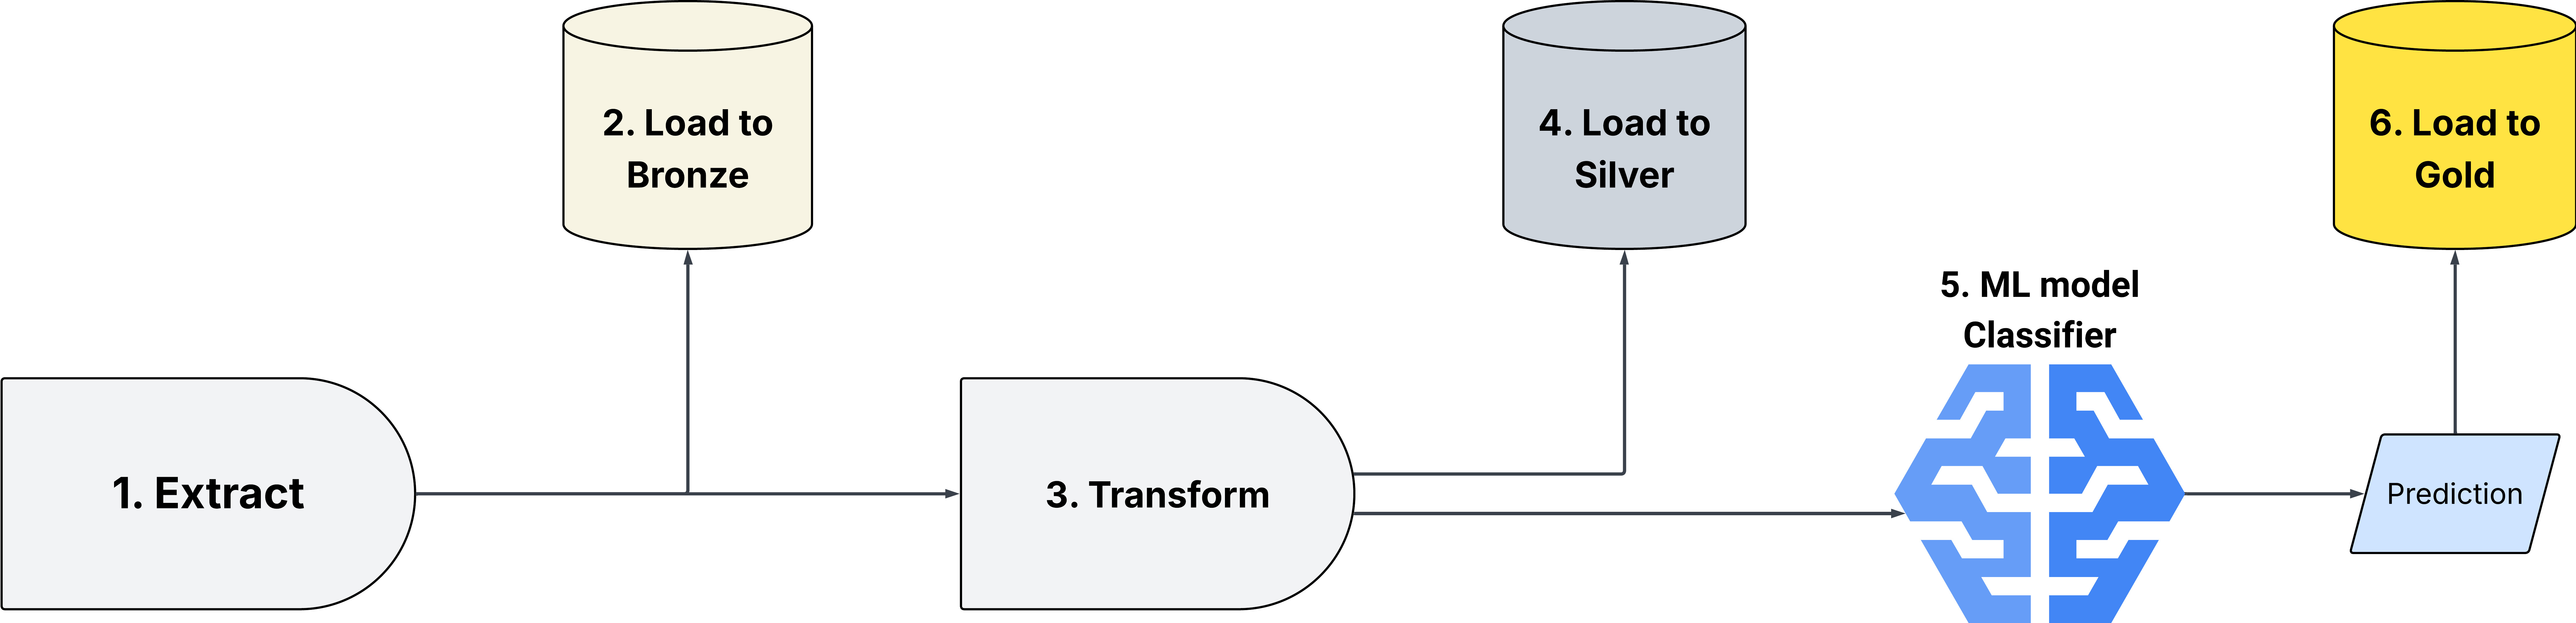
\includegraphics[width=\linewidth]{gfx/examples/medallion.jpeg}
  \caption{Extended ETL Pipeline with Medallion Architecture.}
  \label{fig:medallion}
\end{figure}

\section{ML Layer Design }
Text classification is a core task in Natural Language Processing (NLP) and data mining. It uses machine learning to assign predefined labels to documents so that it provides more context to the text and makes it easier to filter and analyze \cite{allam:2024}.
\smallskip

In the context of this thesis we will frame text classification as supervised machine learning with single-label classification, where the model is trained on a dataset with predefined categories and learns relationships between input and their labels. Afterwards it uses the learned mapping to assign categories or labels to new, unseen texts \cite{wang:2023}.
\smallskip


This module will upgrade the modular ETL pipeline into a full classification pipeline by integrating  ML processes into it. This sub-module is inserted between the silver layer and gold layer, where we use the silver data and perform ML tasks on them.


\subsection{Text classification processes}
Below is a concise overview of all the different stages that the texts goes through before being label. Text classification in practice is not a single model but an evolving process that must keep up with changing data and business goals. Treating it as a set of modular processes helps small teams to upgrade or change one process without disturbing the rest. Here are the key stages the text passes through in our classification pipeline \cite{daud:2023},from clean Silver input to validated predictions logged in Gold.

\begin{enumerate}
  \item Preprocessing
  \item Train/Test Split
  \item Feature Extraction
  \item Model Selection \& Training
  \item Evaluation
  \item Serving
\end{enumerate}

\subsubsection{Preprocessing}
The preprocessing stage cleans and organizes the dataset so it is suitable for classification. Its goal is to reduce noise and inconsistencies and to produce a stable input for the model. The outcome is a structured , conformed dataset that can be safely passed to the training stages. The pre-processing steps performed are defined in here:

\paragraph{Dataset Structuring and Balancing}

\smallskip
In this step we consolidate the textual fields into a single input column. That means if multiple text attributes like for example a news article that has a headline , author and text we merge them into one text. We als standardise labels that may have been written in acronyms or abbreviations into full words.
\smallskip

To address class imbalance, categories which come rarely into the dataset are excluded from modelling. Also from the remaining classes we balance them by reducing the amount of samples to match the size of the smallest represented class \cite{daud:2023}. We record each class counts before and after balancing and visualise distributions to verify the final dataset is suitable for fai evaluation.

\paragraph{Label Encoding}

\smallskip

For modelling task , category labels must be numeric. We apply label encoding to map each distinct class name to an integer id \cite{ahmed:2021}. The resulting integer codes replace the original text labels only in the training data. We persist the mapping of class name to integer with the run metadata so predictions can be decoded back to text labels and experiments are reproducible


\paragraph{Data Preprocessing \& Tokenizing}

\smallskip

We prepare the raw text with a small preprocessing routine so the model sees clean inputs. First, we lowercase all characters so meaning does not depend on letter case. We then remove special characters and digits and normalize whitespaces to single spaces. Next we strip stopwords using a standard list so very common function words do not dominate the representation. Finally we tokenize the text into individual terms and apply light stemming step , so variants like go and going map to a common root. The result is a structured sequence of normalized tokens suitable for downstream feature extraction.


\subsubsection{Train/Test Split}
After feature extraction is defined , we split the dataset into training and test sets to get an unbiased estimate. We use here a 70/30 split where 70\% of data is used for training and 30\% for testing.  We fit the TF-IDF vectorizer on the training dataset only.

\subsubsection{Feature Extraction}
Machine learning models operate on numeric representations, not raw text. Therefore, tokens must be converted into vectors before training. In this study, we use Term Frequency–Inverse Document Frequency (TF-IDF), which is effective for text categorization when word order is less critica \cite{das:2023}. TF-IDF uses two measures:

\begin{itemize}
  \item \textbf{Term Frequency (TF) } how often a term appears in a single document
  \item \textbf{Inverse Document Frequency (IDF): } shows in how many documents a word appears , across the entire dataset

\end{itemize}

\smallskip
We first build a fixed vocabulary from the training data and fit the TF-IDF vectorizer, learning the vocabulary and IDF weights. Each term is assigned a column in the feature space, and each document becomes a row where most entries are zero and the non-zero entries are that document’s TF-IDF weights for the terms present \cite{das:2023}. The fitted vectorizer is then reused to transform validation, test, and future prediction data so the same mapping applies consistently.

\smallskip

Combining TF and IDF balances term importance,where very common words receive lower weights, while more distinctive words receive higher weights. This prevents frequent but less meaningful terms from dominating the model.

\smallskip

After feature extraction, we obtain a sparse TF-IDF document–term matrix with one row per document, the encoded label vector, and the fitted vectorizer containing the vocabulary and IDF weights needed to transform future text into the same feature space.

\subsubsection{Model Selection \& Training}
The pipeline keeps model choice flexible as it accepts any classifier that respects the input-output contract. Based on our literature review we have compiled a list of traditional ML models that can be used for different classification tasks  \cite{allam:2024} :

\begin{table}[htbp]
  \centering
  \begin{tabularx}{\linewidth}{@{}lX@{}}
    \toprule
    \textbf{Model}            & \textbf{Evaluation}                                                                  \\
    \midrule
    Logistic Regresion        & Strong baseline for TF-IDF , fast , interpretable and well-calibrated                \\
    Linear SVM                & Excels on high-dimensional sparse text                                               \\
    Naive Bayes               & Very fast and simple. Works well with word counts.                                   \\
    Random Forest             & Less common for sparse TF-IDF, works better for dense features.                      \\
    K-nearest Neighbors (KNN) & simple and instance based. Works well for small datasets but is slower at interface. \\
    RNN                       & with this model representation of a word depends on the sequence of the tokens.      \\
    Transformers (e.g.\ BERT) & Contextual embeddings. Heavy, but offer the best performance.                        \\
    \bottomrule
  \end{tabularx}
  \caption{Text classification model options .}
  \label{tab:text_cls_models}
\end{table}

After the model of choice was decided we proceed to train it with our chosen dataset. We train models in a simple and repeatable manner. We use the fitted TF-IDF vectorizer to transform training and test data into TF-IDF matrices \cite{daud:2023}. Afterwards it's time to choose the hyperparameters. They control how a model learns and how complex it is \cite{ilemobayo:20243} . Each model has a different set of parameters settings , which we chose before training. Adjusting these values to the given features improve efficiency and accuracy of the model. The process of searching for and selecting the best settings is called hyperparameter tuning \cite{daud:2023}. The last step would be to load the model in a model registry , in the cloud or locally in order to use its prediction function. Now the model is ready for serving and the outcome of this stage is a trained model on a custom dataset ready to be evaluated.


\subsection{Evaluation}
After training the selected classifier , we assess its performance on a series of test metrics. These metrics are used to evaluate the model effectiveness in classifying text with the according label \cite{allam:2024} :

\begin{description}
  \item[Accuracy] measures the share of all predictions that are correct. It is simple and widely used , but can be misleading when classes are imbalanced.
  \item[Precision] measures how many predicted positives are truly positive. It quantifies the purity of positive predictions.
  \item[Recall] measures how many of the actual positives the model correctly identifies. High recall means few missed positives.
  \item[F1-Score] measures the harmonic mean of precision and recall , providing a single score that balances both error types. It is useful with uneven class distribution or when false positives and false negatives both matter.
\end{description}

Taken together all the evaluation metrics provide a view of how well the selected classifier assigns corrects labels. These metrics form the basis for comparing variants of the model.
To connect the results of prediction and evaluation metrics with the data , we write both of them into a predictions table with , \texttt{document\_id}, \texttt{model\_version} , \texttt{hyperparameters}, \texttt{run\_id} and \texttt{predicted\_at}. Because \texttt{document\_id} also exists in Silver layer , we can join predictions with the Silver data to form the Gold data. This keeps raw and cleaned data immutable and enables straightforward comparison across model variants.


\subsection{Serving}
er model training , we expose the model inference in order to communicate with our other system.TensorFlow, a widely used library in the ML ecosystem, is needed for a modular serving system. We separate concerns of  model lifecycle management from the inference execution in order to have a clear modular interface \cite{ilemobayo:20243}:


\begin{description}
  \item[Inference execution] measures the share of all predictions that are correct. It is simple and widely used , but can be misleading when classes are imbalanced.
  \item[Model lifecycle management] measures how many predicted positives are truly positive. It quantifies the purity of positive predictions.
\end{description}

\section{Continuous Learning}

When data distribution shifts over time , static models lose performance. Neural Models trained once on a fixed dataset tend to forget past patterns or overfit to fresh patterns when updated naively. This is called “catastrophic forgetting” \cite{chrysakis:2020}. In order to solve this we need to retrain the model with specific strategy in order to maintain performance as new data comes in. This is an extension of our pipeline which handles pretty advanced topics and the research on this is pretty new , so we will be introducing here today some strategies that can help to continuously feed knowledge to our ML models.
\smallskip

The goal of this section is to design a framework for continuous learning that keeps a ML classifier reliable and performant as data distributions evolve. Concretely we aim to detect performance drift , decide which strategies we should use to retrain the model and set scheduling triggers for retraining. By defining this steps inside the data classification pipeline, we maintain accuracy on our predictions for new data and ensure the system learns from fresh data without forgetting prior knowledge.

\subsection{Detecting data \& performance drift}
We set up parallel monitoring items in order to detect both the data drift from input data and performance drift from prediction outputs.

\paragraph{Detecting Data Drift}
We maintain summaries of each feature and routinely compare recent time windows to a fixed reference set using tests like Population Stability Index (PSI) or KL divergence \cite{cossu:202}. This gives us early warning signals , to measure how far the current feature distribution has moved from the referenced data . We enforce schema and data quality guards like valid ranges or category frequencies to detect pipeline faults. This are needed to detect distribution shifts before they degrade accuracy and provide auditable evidence when and why retraining is needed.

\paragraph{Detecting Performance Drift}
Before learning from new labels,we perform a prequential task , which tests the performance of the next batch before training the mode \cite{cossu:202}. We track common metrics like overall accuracy. We do this not only for the whole batch but for segments of the batch as well to test accuracy on different groups inside the new batch to see if new data , that our model can’t confidently and accurately  predict, exists. With this monitoring items we localize failures in a batch of data and distinguish brief noise from continuous performance degradation.


With data and performance drift monitored we defiance explicit thresholds and log every alert , so that we notice drift signals and make them actionable, to ensure retraining is justified.


\subsection {Retraining strategies}
With our layered data and monitoring in place, we can now select a continuous learning strategy to keep the model robust under data drift. Before choosing , we should define clear objectives, like , target KPIs and metrics , acceptable latency and costs and governance rules for storing historical data. Each strategy group have distinct trade offs in resources , risk and complexity, that’s why we outline the main options in this section [61] :


\subsubsection*{Regularization based}
\begin{description}
  \item[Description] We keep a frozen copy of the last good model as a teacher and while training the new model on new fresh data we add constraints so that its parameters do not drift too far away from the old model’s behavior. We implement a weight regularization function that penalizes the new model if there are big changes in weights.
  \item[Pros] We can retrain frequently because we only need a frozen teacher model in our current training loop which adds small loss. This works as well if we don't want to store historical data , since knowledge distillation can be done on new batches from our teacher model. This produces stable updates with clear auditability because the new model is explicitly tied to the previous one.
  \item[Cons] Can adapt too slowly under hard distribution shifts. Performance is sensitive to hyperparameters like penalty on weight and temperature. If the teacher has errors or biases , the student may inherit them.
  \item[When to use] When we want the simplest safe baseline before adding more complexity to the continuous learning. Useful for frequent , small updates where stability is more important than trying to improve little amounts of accuracy.
\end{description}

\subsubsection*{Replay-based}
\begin{description}
  \item[Description] Replay-based continual learning fights forgetting by rehearsing a small , representative slice of past data , while learning from new data. When we build retraining batches we keep a distribution of 60\% new data and 40\% old data. After each cycle , we refresh the distribution by inserting the most representative newly labeled examples and removing redundant oldest ones. This keeps the class balanced and guard against overfitting.
  \item[Pros] Very efficient against catastrophic forgetting by directly rehearsing on old knowledge. Flexible variants exist if we want to optimize the strategy by changing the distribution of old/new data or other parameters.
  \item[Cons] Needs to be configured on what data to keep and how much. Multiple replays adds training and maintenance overhead and may suffer from quality issues if the data chosen to retrain is not representative.
  \item[When to use] When we care about maximizing accuracy over time when new data comes in this is the best strategy to use. Also when we see that data drift is high and have enough control over data governance then this is a great default for production pipelines once we implement basic data handling policies.
\end{description}

\subsubsection*{Optimization-based}
\begin{description}
  \item[Description] In this method we reduce forgetting by changing how we update the weights, not the model itself. We keep a class-balanced old dataset that represents past knowledge. During each training for each batch of new data we compute a signal if that would harm old performance. If it does we reshape the update so it doesn’t increase old loss.
  \item[Pros] Gives more control over learning so that new learning does not harm old behavior. It can be layered on top of other retraining strategies like replay-based to optimize the model more without changing architecture
  \item[Cons] More compute overhead. Sensitive to implementation details, batching and randomness.
  \item[When to use] We have enough gpu resources and an experienced team.
\end{description}

\subsubsection*{Representation-based}
\begin{description}
  \item[Description] This strategy relies on stable features instead of constantly changing the whole architecture. We use a pre trained encoder and freeze most of the weights. Than learn only small parts like the classifier head , adapters or prompts so the backbone changes little and the representation space stays consistent.  We maintain a class prototype , which is the mean feature per class and use them for calibration or quick checks that the space hasn’t drifted.
  \item[Pros] Fast and low risk updates by relying on stable pretrained encoders and training only a small part of the classifier. Excellent fit for frequent retrains with limited compute power.
  \item[Cons] If the fixed encoder is too frozen , performance can degrade under large data drift.
  \item[When to use] Quick and low-cost updates like weekly or daily scheduling. We already have strong pretrained text encoders and want minimal risk to production.
\end{description}


